\scanpage{26}
\mspage{7}
\figure{
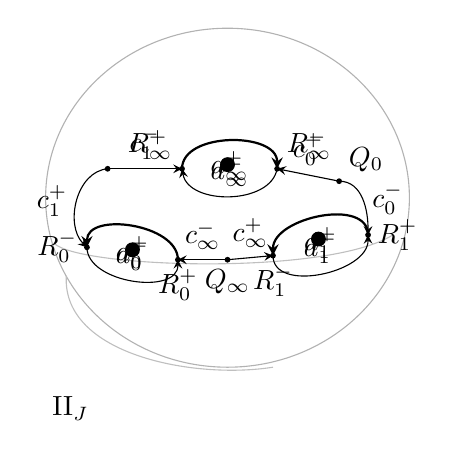
\begin{tikzpicture}[x=1.05cm,y=1.05cm,>=stealth]
\draw[gray!60] (0,.65) ellipse (2.2 and 2.05);
\draw[gray!50] (-2.1,.1) .. controls (-1.8,-.2) and (1.2,-.3) .. (2,.2);
\draw[gray!50] (-1.95,-.3) .. controls (-2,-1.25) and (-.4,-1.55) .. (.55,-1.4);
\coordinate (A) at (-.55,1);\coordinate (B) at (.6,1);
\coordinate (C) at (-1.7,.05);\coordinate (D) at (-.6,-.1);
\coordinate (E) at (.55,-.05);\coordinate (F) at (1.7,.2);
\coordinate (U) at (-1.45,1);\coordinate (V) at (1.35,.85);\coordinate (W) at (0,-.1);
\foreach \p in {A,B,C,D,E,F,U,V,W}{\fill (\p) circle (.035);}
\fill (0,1.05) circle (.09);\fill (-1.15,.02) circle (.09);\fill (1.1,.15) circle (.09);
\draw[->,thick] (A) to[out=90,in=90] node[below] {$a_\infty^+$} (B);
\draw[->] (B) to[out=260,in=280] node[above] {$a_\infty^-$} (A);
\draw[->,thick] (D) to[out=90,in=90] node[below] {$a_0^+$} (C);
\draw[->] (C) to[out=270,in=270] node[above] {$a_0^-$} (D);
\draw[->,thick] (F) to[out=90,in=90] node[below] {$a_1^+$} (E);
\draw[->] (E) to[out=270,in=270] node[above] {$a_1^-$} (F);
\draw[->] (U) to[out=185,in=135] node[left] {$c_1^+$} (C);
\draw[->] (U)--node[above] {$c_1^-$}(A);
\draw[->] (V)--node[above] {$c_0^+$}(B);
\draw[->] (V) to[out=0,in=90] node[right] {$c_0^-$}(F);
\draw[->] (W)--node[above] {$c_\infty^-$}(D);
\draw[->] (W)--node[above] {$c_\infty^+$}(E);
\node[above left] at(A){$R_\infty^+$};\node[above right] at(B){$R_\infty^-$};
\node[left] at(C){$R_0^-$};\node[below] at(D){$R_0^+$};
\node[below] at(E){$R_1^-$};\node[right] at(F){$R_1^+$};
\node[above right] at(V){$Q_0$};\node[below] at(W){$Q_\infty$};
\node at(-1.9,-1.9){$\mathrm{II}_J$};
\end{tikzpicture}
}
On rajoute les sommets $Q_i$ $(i\in J)$ et les arcs
\diagram{\begin{tikzcd}[ampersand replacement=\&]Q_i\arrow[r,"c_i^\omega"]\&R_{\omega'i}^{\omega'}\end{tikzcd}}
permutés \deleted{de façon \unsure{simplement} \unsure{transitivement}} par $G_J$. On a maintenant
\[
(13)\qquad b_i^\omega=c_i^\omega(c_i^{\omega'})^{-1}
\]
(donc les $b_i^\omega$ deviennent inutiles comme générateurs d'un groupoïde). \inserted{\unsure{Dans}} Les relations \inserted{$(2)$} \deleted{deviennent} la partie $(a)$ devient automatique, pour écrire commodément la partie $(b)$, \unsure{on} introduit les
\[
(14)\qquad\widetilde a_i^\omega=
\deleted{(\unsure{c_{\omega i}^{\omega}})^{-1}a_i^{\unsure{\omega}}\unsure{c_{\omega'i}^{\omega'}}}
\inserted{(c_{\omega i}^\omega)^{-1}a_i^\omega c_{\omega'i}^{\omega'}}
:\quad Q_{\omega'i}\longrightarrow Q_{\omega i}
\]
\diagram{
\begin{tikzcd}[ampersand replacement=\&,column sep=small,row sep=large]
Q_{\omega i}\&R_i^{\omega'}\arrow[l,"(c_{\omega i}^{\omega})^{-1}"']\arrow[r,dashed,bend right=28,"a_i^{\omega'}"']\&R_i^\omega\arrow[l,bend right=45,"a_i^\omega"']\&Q_{\omega'i}\arrow[l,"c_{\omega'i}^{\omega'}"]\\
\deleted{\unsure{Q_{\omega i}}}\arrow[r,"\deleted{\unsure{c_{\omega i}^{\omega}}}"]\&\deleted{\unsure{R_i^\omega}}\arrow[r,bend right=45,"\deleted{a_i^{\omega'}}"']\&\deleted{\unsure{R_i^{\omega'}}}\arrow[r,"\deleted{(c_{\omega'i}^{\omega'})^{-1}}"']\&\deleted{\unsure{Q_{\omega'i}}}
\end{tikzcd}}
\margin{\figure{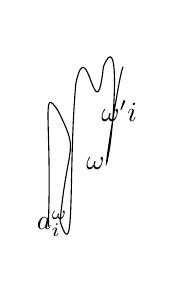
\begin{tikzpicture}[x=.5cm,y=.7cm]
\draw (0,0) .. controls (.1,1.9) and (-.2,2.6) .. (.25,2.1) .. controls (.8,1.3) and (.5,1.6) .. (.3,.1);
\draw (.3,.1) .. controls (.7,-.8) and (.5,1) .. (.7,2.6) .. controls (1,3.6) and (1.2,1.6) .. (1.4,2.9) .. controls (1.8,3.6) and (1.7,2.1) .. (1.55,1.4) .. controls (1.3,.4) and (1.8,2.8) .. (1.9,2.9);
\node at(.1,.05){$\unsure{a_i^\omega}$};\node at(1.2,1.15){$\unsure{\omega}$};\node at(1.8,2.1){$\unsure{\omega'i}$};
\end{tikzpicture}}}
qui sont également permutés de façon simpl. transitive sous $G_J$, et on a
\[
(15)\qquad\tau(\widetilde a_i^\omega)=(\widetilde a_i^{\omega'})^{-1}
\]
La relation $(2b)$ devient
\[
(16)\qquad\widetilde a_{\unsure{\omega^2i|\omega'i}}^\omega\widetilde a_{\omega i}^\omega\widetilde a_i^\omega=1
\]
(deux relations ess\textsuperscript{t.} distinctes qui sont permutées par $\tau$)

Pour repérer les \inserted{$\pi(Q_i)=$} $\pi_1(\Sigma_J(\mathbb C),Q_i)$ de façon commode on utilise les
\diagram{
\begin{tikzcd}[ampersand replacement=\&,column sep=large,row sep=large]
(17)\quad\psi_i^\omega:\ \deleted{\unsure{Q}}\Pi_{0,3}\arrow[rr,"\sim"]\arrow[dr,"\varphi_{\omega'i}^{\omega'}"',"\sim"]\&\&\pi(Q_i)\\
\&\pi(R_{\omega'i}^{\omega'})\arrow[ur,"(c_i^\omega)^{-1}"',"\sim"]\&
\end{tikzcd}}
\margin{\uline{NB}\quad$\tau\psi_i^\omega(g)=\psi_i^\omega(\tau_\infty g)$}
on aura
\[
(18)\qquad\psi_i^\omega(g)=\psi_i^{\omega'}(\sigma_\infty(g))
\]
\[
(19)\qquad\begin{aligned}
\widetilde a_i^{\unsure{\omega|\omega^*}}(\psi_{\omega'i}^{\omega'}(g))
&=\psi_{\unsure{\omega i}}^{\unsure{\omega}}(\varepsilon_0(g))
=\psi_{\unsure{\omega i}}^{\omega'}(\overbrace{\sigma_\infty\varepsilon_0}^{\deleted{\unsure{\xi}}\tau_\infty(\rho)}(g))\\
\boxed{\widetilde a_i^\omega(\psi_{\omega'i}^{\omega}(g))
=\psi_{\unsure{\omega i}}^{\unsure{\omega}}(\overbrace{\varepsilon_0\sigma_\infty}^{\rho^{-1}}(g))}
=\psi_{\omega i}^{\omega'}(\sigma_\infty\varepsilon_0\sigma_\infty(g))
\end{aligned}
\]
\margin{25}
